\subsubsubsection{Bootstrap}
In order to neatly start the application layer, we have to consider the 
dependencies among the entity types exposed in \ref{fig:sd-entity-types-deps}. 
Moreover we have to take into account that this layer can not decide by itself 
when it is time to boot, indeed it is ruled by the middleware one.
The bootstrap of the application layer needs a \textit{master} process, 
which has to create the entities based on the configuration provided by 
the middleware layer. 
Bearing in mind the mentioned dependencies:
\begin{itemize}
  \item The \textit{reactive} entities have to start before the \textit{active} 
ones, because the latter use the former; 
  \item The \textit{passive} entities have no particular dependency. Since 
they are stateless and they logically belong to \textit{reactive} entities 
(e.g. the road signs belong to roads), they have to be instantiated along with them.
\end{itemize}

\begin{figure}[H]
  \centering
  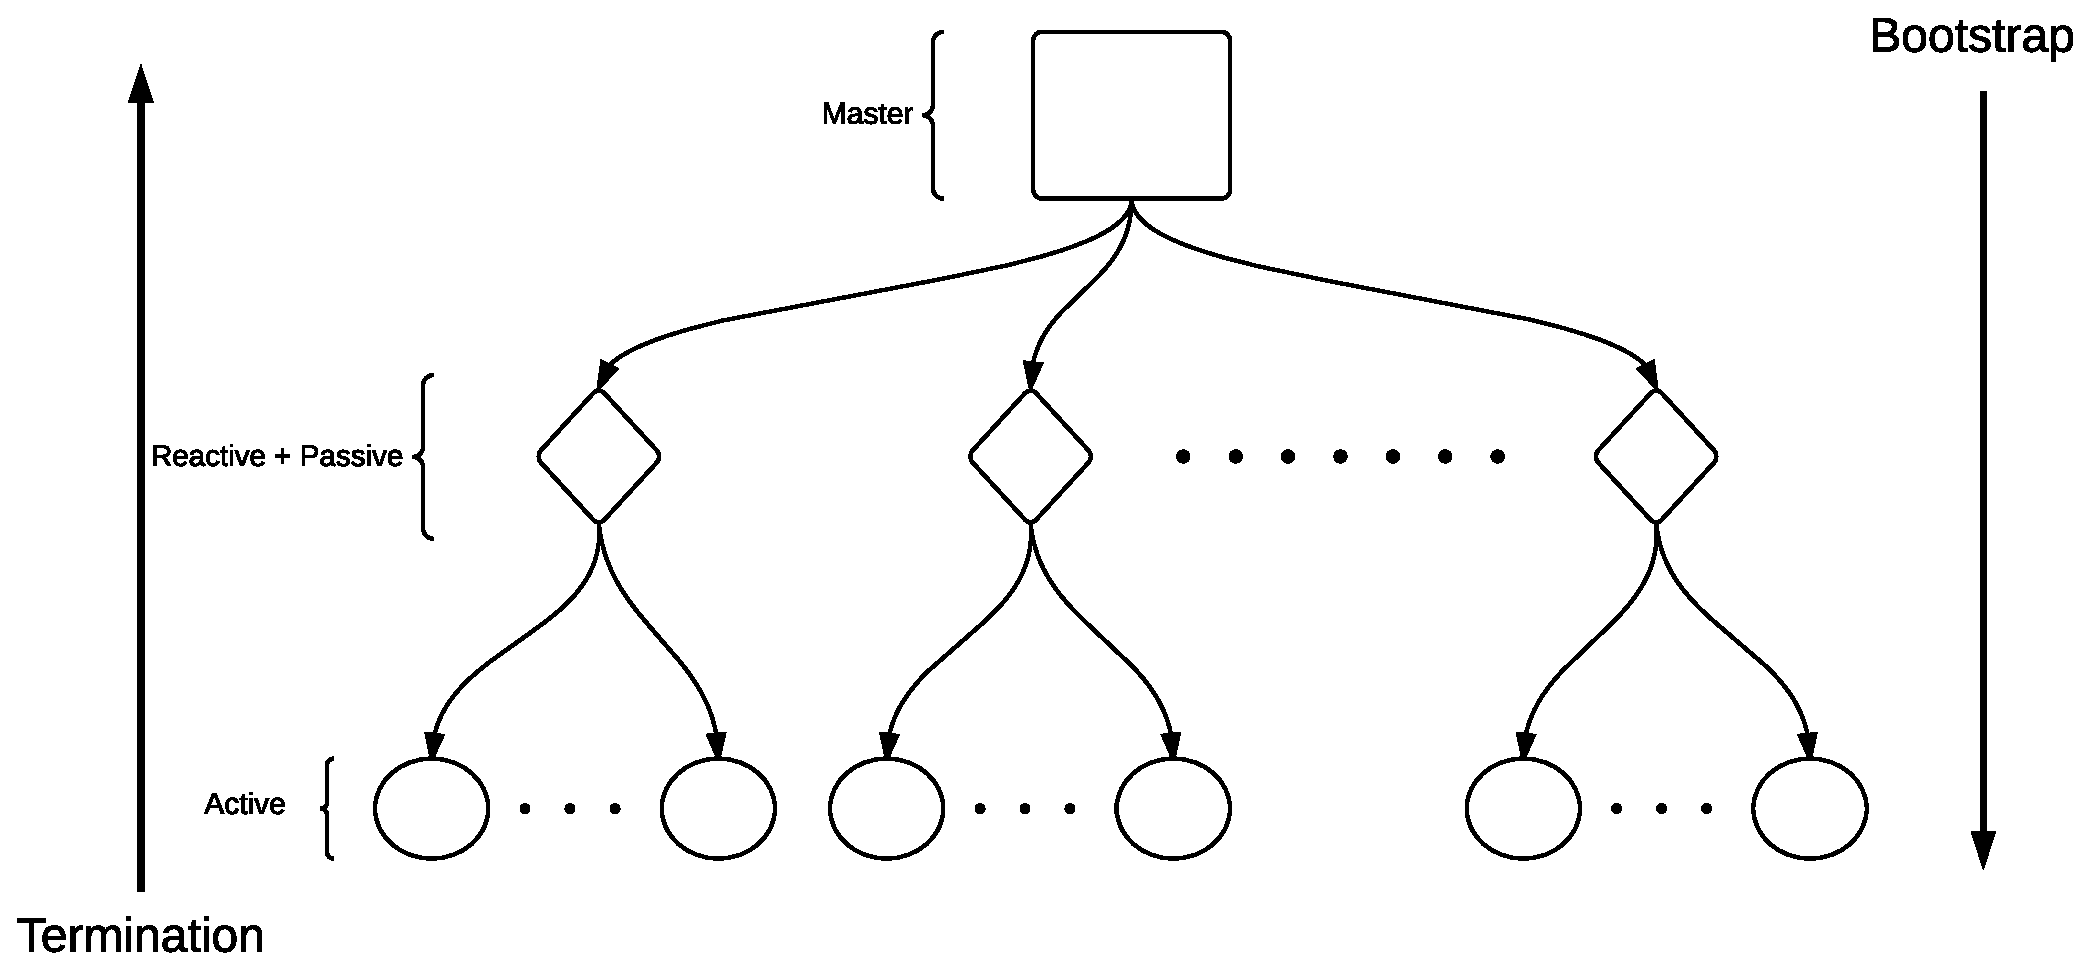
\includegraphics[width=\columnwidth]{sections/images/solution/app_proc_tree.eps}
  \caption{Application process tree}
  \label{fig:app-proc-tree}
\end{figure}

At the end of the bootstrap, the \textit{master} process has to notify the 
middleware layer of the successful completion. A crash of the
\textit{master} process, occurring before the end of the bootstrap, 
is signaled to the middleware layer, because of the expiration 
of the timeout attached to the \texttt{app.boot} call. 
Note that this model works also for a bootstrap which is executed starting 
from a snapshot of the system, with the only difference consisting in divergent
values of the configuration file. Indeed, we have to use a set of 
configurations, which is different for each city.